\documentclass[a4paper,10pt]{article}

\usepackage{graphicx}
\usepackage[utf8]{inputenc}
\usepackage[T1]{fontenc}
\usepackage{wrapfig}

\usepackage{hyperref}
\setlength{\parindent}{10pt}
\setlength{\parskip}{1.5mm}
\usepackage{geometry}
\geometry{margin=1.25cm}
\addtolength{\textheight}{-1.5cm}
\setlength{\headheight}{32pt}

\usepackage{amsfonts, amstext, color,
	ifthen, fancybox, multirow, fancyhdr, pgf, tikz,%
	colortbl, array, tabularx
}

\definecolor{bgcode}{rgb}{0.95,0.95,0.95}

\usepackage{url}

\usepackage[french]{babel}
\selectlanguage{french}

%partie concernant la gestion des entêtes
\usepackage{fancyhdr}
\pagestyle{fancy}
\usepackage{lastpage}
\renewcommand\headrulewidth{1pt}
\fancyhead[L]{Interface Homme-Machine Android}
\fancyhead[R]{Université de Poitiers}
\renewcommand\footrulewidth{1pt}
\fancyfoot[L]{Département d'Informatique}
\fancyfoot[C]{\textbf{\thepage/\pageref{LastPage}}}
\fancyfoot[R]{année 2024-2025}
%fin

\usepackage{enumitem}

\usepackage{listings}

\usepackage{version}
\usepackage{tcolorbox}

\newcounter{Exercice}
\newcommand{\Exercice}[1]{\refstepcounter{Exercice}%
	\ \vspace{0mm} \\ \hspace{0.8cm}%
	\noindent \hspace*{0.5cm} {\bf Question \theExercice :} #1 \vspace{-13mm} \\ %
	\subparagraph*{}%
}

\lstset{language=Caml,basicstyle=\normalsize\tt,keywordstyle=\ttfamily\bfseries\underbar,%
	commentstyle=\normalsize, extendedchars=true, fontadjust=true, columns = flexible, flexiblecolumns=true,
	linewidth=.975\linewidth, backgroundcolor=\color{bgcode}, frame=tlrb, xleftmargin=1cm}

\lstnewenvironment{ocamlcode}
{\lstset{language=Caml,basicstyle=\normalsize\tt,keywordstyle=\ttfamily\bfseries\underbar,%
		commentstyle=\normalsize, extendedchars=true, fontadjust=true, columns = flexible, flexiblecolumns=true,
		linewidth=.975\linewidth, backgroundcolor=\color{bgcode}, frame=tlrb, xleftmargin=1cm,
		literate={à}{{\`a}}1 {è}{{\`e}}1 {é}{{\'e}}1 {ê}{{\^e}}1,
	}}%, framexleftmargin=5mm,frame=box}}
{}

\lstnewenvironment{fsharp}
{\lstset{language=Caml,basicstyle=\normalsize\tt,keywordstyle=\ttfamily\bfseries\underbar,%
		commentstyle=\normalsize, extendedchars=true, fontadjust=true, columns = flexible, flexiblecolumns=true,
		linewidth=.975\linewidth, backgroundcolor=\color{bgcode}, frame=tlrb, xleftmargin=1cm,
		literate={à}{{\`a}}1 {è}{{\`e}}1 {é}{{\'e}}1 {ê}{{\^e}}1 {ç}{{\c c}}1,
}}%, framexleftmargin=5mm,frame=box}}
{}

\lstnewenvironment{javasansbord}
{\lstset{language=Java,basicstyle=\normalsize\tt,keywordstyle=\ttfamily\bfseries\underbar,%
		commentstyle=\normalsize, extendedchars=true, fontadjust=true, columns = flexible, flexiblecolumns=true,
		linewidth=.975\linewidth,frame=,backgroundcolor=,xleftmargin=0cm,
		literate={à}{{\`a}}1 {è}{{\`e}}1 {é}{{\'e}}1 {ê}{{\^e}}1 {ç}{{\c c}}1,
}}%, framexleftmargin=5mm,frame=box}}
{}

\lstnewenvironment{java}
{\lstset{language=Java,basicstyle=\normalsize\tt,keywordstyle=\ttfamily\bfseries\underbar,%
		commentstyle=\normalsize, extendedchars=true, fontadjust=true, columns = flexible, flexiblecolumns=true,
		linewidth=.975\linewidth, backgroundcolor=\color{bgcode}, frame=tlrb, xleftmargin=1cm,
		literate={à}{{\`a}}1 {è}{{\`e}}1 {é}{{\'e}}1 {ê}{{\^e}}1 {ç}{{\c c}}1,
}}%, framexleftmargin=5mm,frame=box}}
{}

\lstnewenvironment{csharpsansbord}
{\lstset{language=[Sharp]C,basicstyle=\normalsize\tt,keywordstyle=\ttfamily\bfseries\underbar,%
		commentstyle=\normalsize, extendedchars=true, fontadjust=true, columns = flexible, flexiblecolumns=true,
		linewidth=.975\linewidth,frame=,backgroundcolor=,xleftmargin=0cm,
		literate={à}{{\`a}}1 {è}{{\`e}}1 {é}{{\'e}}1 {ê}{{\^e}}1 {ç}{{\c c}}1,
}}%, framexleftmargin=5mm,frame=box}}
{}


\newboolean{versionenseignant}
%%%%%%%%%%%%%%%%%%%%%%%%%%%%%%%%%%%%%%%%%%%%%%%%%%%%%%%%%%%%%%%%%%%%%%%%%%%%%%%%%%%%%%%%%%%%%%%%%%%%%%%%
%__     __            _
%\ \   / /__ _ __ ___(_) ___  _ __
% \ \ / / _ \ '__/ __| |/ _ \| '_ \
%  \ V /  __/ |  \__ \ | (_) | | | |
%   \_/ \___|_|  |___/_|\___/|_| |_|
% _____                _                         _
%| ____|_ __  ___  ___(_) __ _ _ __   __ _ _ __ | |_
%|  _| | '_ \/ __|/ _ \ |/ _` | '_ \ / _` | '_ \| __|
%| |___| | | \__ \  __/ | (_| | | | | (_| | | | | |_
%|_____|_| |_|___/\___|_|\__, |_| |_|\__,_|_| |_|\__|
%                        |___/ 
%% modifiez le booleen ci-dessous pour generer la version enseignant ou etudiant
%% ===> true = version enseignant
%% ===> false = version etudiant
\setboolean{versionenseignant}{false}
%%%%%%%%%%%%%%%%%%%%%%%%%%%%%%%%%%%%%%%%%%%%%%%%%%%%%%%%%%%%%%%%%%%%%%%%%%%%%%%%%%%%%%%%%%%%%%%%%%%%%%%%
% \includeversion{ensnote}
%\excludeversion{ensnote}
\ifthenelse{\boolean{versionenseignant}}{\includeversion{ensnote}}{\excludeversion{ensnote}}

\tcbuselibrary{breakable}


\newenvironment{solution}%
{\begin{tcolorbox}[breakable,colback=red!5!white,colframe=red!75!black,title=Solution]}%
{\end{tcolorbox}}

%\tcblower

\newenvironment{info}%
{\begin{tcolorbox}[breakable,colback=green!5!white,colframe=green!75!black,title=Information]}%
{\end{tcolorbox}}


\newenvironment{attention}%
{\begin{tcolorbox}[breakable,colback=green!25!white,colframe=red!55!black,title=Attention]}%
{\end{tcolorbox}}


\newenvironment{boxcode}%
{\begin{tcolorbox}[breakable,colback=gray!5!white,colframe=black]}%
	{\end{tcolorbox}}
	
	
\begin{document}
	


\title{\vspace*{-1cm}Manipulation des layouts}
\author{\vspace*{-1.5cm}Interface Homme-Machine: Unity
\begin{ensnote}
	(Version enseignant)
\end{ensnote}
}
\date{\vspace*{-1.5cm}version 1}
\maketitle
\thispagestyle{fancy}

Voici les objectifs de ce sujet:
\begin{itemize}
	\item continuer à manipuler l'IDE \texttt{Unity};
	\item continuer la création d'un \textit{widget} complexe;
	\item exploiter les mécaniques vues précédemment;
	\item utiliser les \texttt{Layouts}.
\end{itemize}


%\begin{attention}
%	Le sujet ce fait en deux étapes. Avec une proposition notée de votre interface au bout de 2h (si vous avez fini avant la \textit{deadline} rien ne vous empêche de continuer)!
%	
%	N'oubliez pas d'utiliser les bons réflexes de tout développeur:
%	\begin{itemize}
%		\item Le système de log très bien fait sous Android
%		\item Le mode débogue qui vous permet de voir les valeurs des variables pendant 
%	\end{itemize}
%\end{attention}

\section{Description générale du TP}

La fois précédente, nous avons réalisé nos premiers widgets complexes en exploitant l'agrégation de plusieurs widgets de base. Nous avons en particulier manipulé le système d'ancre que propose \texttt{Unity} pour placer les objets de façon relative.

Dans ce TP, nous allons employer une autre méthode un peu plus coûteuse mais offrant une plus grande puissance en terme de placement et qui reprend les points que vous avez étudié durant les années précédentes en IHM: les mises en page (\texttt{layouts}). La documentation est présente ici: \url{https://docs.unity3d.com/Packages/com.unity.ugui@1.0/manual/UIAutoLayout.html}

\ifversionenseignant
\begin{solution}
Créer un nouveau projet de type \texttt{Universal 3D Core}.
	
\end{solution}
\fi 

\subsection*{Composants basiques}

\begin{itemize}
	  \item Tester les propriétés du  composant \texttt{Content Size Fitter} sur un \texttt{GameObject} de type \texttt{Text} ou \texttt{Image}.
	  
\ifversionenseignant
\begin{solution}
Source : \href{https://docs.unity3d.com/Packages/com.unity.ugui@1.0/manual/script-ContentSizeFitter.html}{Doc. Content Size Fitter}.\\

Ce \texttt{Component} permet de gérer les dimensions du \texttt{Component} auquel il est rattaché (pas celui de ses enfants).

\begin{itemize}
	\item Créer un \texttt{Canvas} et y ajouter un \texttt{Panel}.
	\item Dans ce \texttt{Panel}, créer un \texttt{GameObject Text (Legacy)}.
	\item Associer à ce \texttt{Text} un \texttt{Component Content Size Fitter}.
	\item Tester ses propriétés:
	\begin{itemize}
		\item 	\texttt{Unconstrained} : on peut redimensionner le \texttt{Text} comme on le souhaite;
		\item \texttt{Min Size} : fixe les dimensions aux valeurs minimum du \texttt{Text} $\Rightarrow$ attention, ces valeurs valent 0;
		\item \texttt{Preferred Size} : adapte les dimensions du \texttt{Text} à son contenu ; tester avec différentes tailles de fonte (par exemple 60).		
	\end{itemize}	
\end{itemize}

\end{solution}
\fi 
	  
	  \item Faites de même pour le composant \texttt{Aspect Ratio Filter}. Pour bien distinguer les effets de chaque composant, il est recommandé d'en associer un seul à la fois au \texttt{GameObject}.
	  
\ifversionenseignant
\begin{solution}
	Source : \href{https://docs.unity3d.com/Packages/com.unity.ugui@1.0/manual/script-AspectRatioFitter.html}{Doc. Aspect Ratio Fitter}.
	
	\begin{itemize}
		\item Retirer le composant \texttt{Content Size Fitter} du \texttt{Text} précédent.
		\item Ajouter le composant \texttt{Aspect Ratio Fitter} au \texttt{Text}.
		\item Tester ses propriétés:
		\begin{itemize}
			\item 	\texttt{Width Controls Height} : la hauteur est calculée à partir de la valeur de la largeur, selon le coefficient multiplicateur \texttt{Aspect Ratio} (largeur divisée par hauteur);
			\item \texttt{Height Controls Width} : c'est l'inverse			
			\item \texttt{Fit In Parent} : le \texttt{Text} est agrandi jusqu'à ce que sa largeur ou sa hauteur atteigne celle de son parent (ici, le \texttt{Panel}); \texttt{Aspect Ratio} est toujours modifiable.
			\item\texttt{ Envelope Parent} redimensionne le \texttt{Text} jusqu'à recouvrir son parent. Selon \texttt{Aspect Ratio}, cela peut entraîner le dépassement du composant par rapport à son parent.
		\end{itemize}	
	\end{itemize}
	
\end{solution}
\fi 
	  
\end{itemize}

\section{Présentation des outils de mise en pages en Unity UI}

Il est conseillé de lire en détail la documentation citée plus haut pour bien comprendre les aspects des composants. Voici le résumé des points-clés:
\begin{itemize}
	\item Il y a deux types de composants dédiés à la mise en page.
	\item Les \textit{conteneurs} ou \texttt{Layout Group} contrôlent le comportement des widgets enfants (enchaînement horizontal, enchaînement vertical ou sous forme de grille\ldots)
\begin{center}
	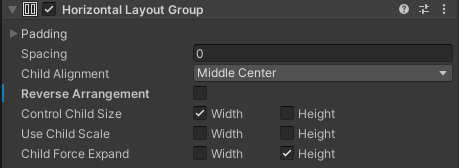
\includegraphics[width=0.6\linewidth]{rc/ui_layout_group_horiz}
\end{center}	
	\item Les composants \textit{éléments} ou \texttt{Layout Element} qui précisent les propriétés de mise en page.
\begin{center}
	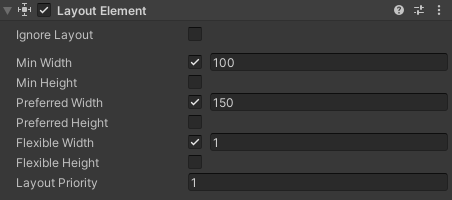
\includegraphics[width=0.6\linewidth]{rc/ui_layout_element}
\end{center}
\end{itemize}

Ainsi, chaque conteneur peut avoir des paramétrages différents qui vont faire évoluer les éléments selon les contraintes. Vous ferez attention à certains paramètres qui peuvent forcer le redimensionnement des \texttt{widgets} éléments sans les consulter. Vous prendrez également garde aux éléments qui doivent activer la flexibilité des dimensions voulues pour agrandir dans cette direction (une valeur de 1 peut être suffisante pour indiquer un degré de liberté).

\subsection*{Tests}

\begin{enumerate}
	\item Dans un premier temps, tester les conteneurs \texttt{Horizontal Layout Group}, \texttt{Vertical Layout Group} et \texttt{Grid Layout Group} \textbf{sans} ajouter de composant \texttt{Layout Element} aux enfants des groupes.
	
\ifversionenseignant
\begin{solution}
	\paragraph{Horizontal Layout Group}
	
	Source : \href{https://docs.unity3d.com/Packages/com.unity.ugui@1.0/manual/script-HorizontalLayoutGroup.html}{Doc. Horizontal Layout Group}.
	
	\begin{itemize}
		\item Supprimer le \texttt{Text} précédent et en ajouter un nouveau dans le \texttt{Panel}.
		\item Ajouter un \texttt{Slider} dans le \texttt{Panel} et le déplacer pour le mettre à côté de \texttt{Text}.
		\item Ajouter au \texttt{Panel} le composant \texttt{Horizontal Layout Group} : les enfants sont automatiquement replacés dans le \texttt{Child Alignment} par défaut : \textit{Upper Left}.
		\item Modifier les propriétés de ce composant:
		\begin{itemize}
			\item \texttt{Padding} : espacement par rapport au bord du \texttt{Panel}
			\item \texttt{Spacing} : espacement entre les \texttt{GameObject} enfants
			\item \texttt{Child Alignment} (\texttt{Upper Left} par défaut) : alignement des enfants
			\item \texttt{Reverse Alignment} : inverse l'ordre des enfants
			\item \texttt{Control Child Size} : modifie les dimensions des enfants en fonction de celles du parent (les propriétés de dimension et de position du \texttt{Rect Transform} des enfants sont bloquées).
			\item \texttt{Use Child Scale} : détermine si l'échelle de redimensionnement des enfants est prise en compte dans leur redimensionnement $\Rightarrow$ tester les effets de cette propriété lorsque les propriétés \texttt{Rect Transform > Scale} des enfants sont différentes de 1.
			\item \texttt{Child Force Expand} : force les enfants à se redimensionner pour occuper l'espace utilisable dans le parent.
		\end{itemize}	
	\end{itemize}
	
\paragraph{Vertical Layout Group}

Source : \href{https://docs.unity3d.com/Packages/com.unity.ugui@1.0/manual/script-VerticalLayoutGroup.html}{Doc. Vertical Layout Group}.

Même procédure que pour le composant \texttt{Horizontal Layout Group}.

\paragraph{Grid Layout Group}

Source : \href{https://docs.unity3d.com/Packages/com.unity.ugui@1.0/manual/script-GridLayoutGroup.html}{Doc. Grid Layout Group}.

	\begin{itemize}
	\item Retirer le \texttt{Layout Group} précédent du \texttt{Panel}.
	\item Insérer d'autres widgets dans ce \texttt{Panel} et les disposer librement.
	\item Associer le composant \texttt{Grid Layout Group} au \texttt{Panel} et modifier ses propriétés
	\begin{itemize}
		\item \texttt{Padding} : cf. plus haut
		\item \texttt{Cell Size} : définit les dimensions des enfants
		\item \texttt{Start Corner}: le coin où le premier enfant est placé
		\item \texttt{Start Axis} : sélectionne l'axe de placement principal (horizontal ou vertical)
		\item \texttt{Child Alignment}: alignement des enfants s'ils ne remplissent pas tout l'espace disponible
		\item \texttt{Constraint}: précise le nombre de lignes et de colonnes à respecter. La valeur \textit{Flexible} redispose les enfants selon le redimensionnement du parent.
	\end{itemize}	
\end{itemize}

\end{solution}
\fi 
	
	
	\item Associer ensuite des \texttt{Layout Element} aux enfants des groupes et tester les conteneurs.

	
\ifversionenseignant
\begin{solution}
	\paragraph{Layout Element}
	
Ce composant est ajouté aux enfants eux-mêmes et leurs propriétés se combinent avec celles des\texttt{ Layout Group} de leur parent. Les propriétés d'un \texttt{Layout Element} sont : 
\begin{itemize}
	\item \texttt{Ignore Layout} : le \texttt{Layout} est ignoré (pratique si les réglages entrent en contradiction avec ceux d'un parent);
	\item \texttt{Min Width, Min Height} : dimensions minimales de cet élément;
	\item \texttt{Preferred Width, Preferred Height} : dimensions préférées de cet élément. La valeur affectée est calculée en fonction du contenu existant;
	\item \texttt{Flexible Width, Flexible Height} : valeur relative disponible pour que l'élément courant se redimensionne par rapport à ses frères;
	\item  \texttt{Layout Priority} : si le \texttt{GameObject} est associé à plusieurs composants qui disposent chacun de propriétés de Layout, il faut éviter que ces dernières interfèrent. Le composant disposant de la priorité maximale prend le pas sur les autres.	
\end{itemize}

Remarque : certaines propriétés peuvent interférer avec celles du parent. Par exemple, si on utilise un \texttt{Grid Layout Group} qui fixe les dimensions des cellules, les propriétés de dimension des éléments de ce groupe devraient être recalculées (voir l'effet avec \texttt{Preferred Width/Height} par exemple).	
\end{solution}
\fi 

	
	
\end{enumerate}

\section{Widget: ComplexSlider - le retour en joli}

Refaites le widget \texttt{ComplexSlider} (soit sous un autre nom, soit après avoir fait une sauvegarde de votre ancien projet/widget). Pour obtenir un affichage joli, peu importe la largeur que vous donnerez à votre widget, pourvu que le \texttt{Slider} prenne la plus grande place.

Veillez à ce que le widget contenant la valeur numérique ne soit pas modifiable directement par l'utilisateur.

\begin{center}
	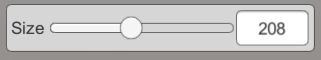
\includegraphics[width=0.6\linewidth]{rc/ui_complexslider_layout}

	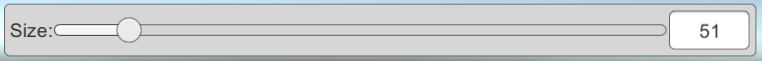
\includegraphics[width=0.8\linewidth]{rc/ui_complexslider_layout_v2}
	
\end{center}


\ifversionenseignant
\begin{solution}
	\subsection{Création du ComplexSliderJoli}
Le principe est de recréer un \texttt{Complex Slider} nommé \textit{ComplexSliderJoli} tel que les dimensions du \texttt{Text} à gauche du \texttt{Slider} et du \texttt{Input Field} à droite soient conservées, tandis que le \texttt{Slider} au centre est redimensionné en même temps que le \texttt{Panel}.\\

Important: vérifier que le \texttt{Canvas} ne possède aucun \texttt{Group Layout}, pour éviter qu'il n'interfère avec les étapes suivantes.\\

Commencer par insérer un \texttt{Panel} dans le \texttt{Canvas} avec \texttt{UI > Panel}.

Dans ce \texttt{Panel}, créer un nouveau \texttt{Panel} nommé \textit{ComplexSliderJoli}, insérer
un composant \texttt{Horizontal Layout Group} et
des enfants \texttt{Text (Legacy)}, \texttt{Slider} et \texttt{InputField (Legacy)}.
Noter que ces enfants sont automatiquement disposés en haut à gauche du \texttt{Panel} (réglage par défaut du Horizontal \texttt{Layout Group > ChildAlignment : Upper Left}).

\begin{itemize} 
\item \texttt{Text}
	\begin{itemize} 	
		\item modifier les propriétés
		\begin{itemize} 	
			\item \texttt{Text > Text} : \textit{Size}
			\item \texttt{Text > Character > Font Size} : $42$ (\textbf{attention} : cette taille est trop grande pour loger le texte : ce dernier n'apparaît pas actuellement)
			\item \texttt{Text > Paragraph > Alignment} : \textit{Center / Middle}
		\end{itemize}	
		\item ajouter le composant \texttt{Layout Element} avec les propriétés
		\begin{itemize} 	
			\item \texttt{Min Width} (cochée) : $160$
			\item \texttt{Preferred Width} (cochée) : $160$
		\end{itemize}	
	\end{itemize}
\item \texttt{Slider}
\begin{itemize} 	
	\item modifier les propriétés du composant \texttt{Slider}
	\begin{itemize}
		\item \texttt{Min Value} : $0$
		\item \texttt{Max Value} : $999$
		\item \texttt{Whole Numbers} : cocher
	\end{itemize}			
	\item enfant \texttt{Handle Slide Area > Handle} : dans \texttt{Rect Transform}, modifier la propriété \textit{Width} pour la rendre égale à la hauteur  du \texttt{Slider}.
	\item ajouter le composant \texttt{Layout Element} avec les propriétés
	\begin{itemize}
		\item \texttt{Min Width} (cochée) : $100$
		\item \texttt{Flexible Width} (cochée) : $1$
		\item \textbf{Important}: C'est cette propriété \texttt{Flexible Width} qui active le redimensionnement du \texttt{Slider} en même temps que celui du \texttt{Panel} parent \texttt{ComplexSliderJoli}. 
	\end{itemize}	
\end{itemize}
\item \texttt{InputField}
	\begin{itemize} 	
		\item propriété \texttt{Interactable} : désactiver pour empêcher l'utilisateur d'écrire dans ce champ;
		\item propriété \texttt{Transition > Disabled Color} : cette couleur est gris par défaut, passer cette couleur en \textit{blanc} et \textit{alpha = 255} pour suivre l'illustration du sujet;
		\item composant \texttt{Text} : modifier les propriétés
		\begin{itemize} 	
			\item \texttt{Text > Text} : \textit{000} (ou bien directement dans le \texttt{Input Field} lui-même),
			\item \texttt{Text > Character > Font Size} : $30$ (pas forcément visible par défaut, il faudra augmenter la taille du parent au besoin -- $50$ par exemple),
			\item \texttt{Text > Paragraph > Alignment} : \textit{Center / Middle}
		\end{itemize}		
		\item ajouter le composant \texttt{Layout Element} avec les propriétés
		\begin{itemize} 	
			\item \texttt{Min Width} (cochée) : $160$
			\item \texttt{Preferred Width} (cochée) : $160$
		\end{itemize}		
	\end{itemize}	
\end{itemize}



\begin{itemize} 	
	\item  \texttt{ComplexSliderJoli}
	\begin{itemize} 	
		\item Propriétés du \texttt{Horizontal Layout Group}:
		\begin{itemize} 
			\item \texttt{Spacing} : jouer sur cette valeur pour que la poignée du \texttt{Slider} ne chevauche pas les autres \texttt{widgets} lors de son déplacement aux extrémités.	
			\item \texttt{ChildAlignment}: conserver \texttt{Upper Left}
			\item \texttt{Control Child Size > Height / Width} : valider les deux valeurs pour redimensionner les enfants en fonction de la taille de \texttt{ComplexSliderJoli} (plus précisément, la hauteur de tous les enfants sera affectée ; mais seule la largeur du \texttt{Text} et du \texttt{InputField} ne sera pas modifiée, car la propriété \texttt{Flexible Width} de leur composant \texttt{Layout Element} n'est pas cochée).
			\item \texttt{Child Force Expand} : cocher \texttt{Height} et décocher \texttt{Width} pour adapter la hauteur (pas la largeur) des enfants à celle de leur parent.		
		\end{itemize}	
		\item \texttt{Rect Transform} : si la largeur (\texttt{Width}) et/ou la hauteur (\texttt{Height}) est passée à $0$ lors des dernières manipulations, fixer ces valeurs, par exemple \textit{800x600}. En jouant sur ces valeurs (outil \texttt{Rect Tool} dans la fenêtre glissante sur la \texttt{Scene}), on valide bien le redimensionnement en largeur du \texttt{Slider} uniquement.
	\end{itemize}
\end{itemize}

Remarque : les composants de type \texttt{Text} nécessitent une taille minimale pour que leur contenu soit visible. Attention en redimensionnant le parent...

\subsection{Script à associer au ComplexSliderJoli}

\begin{boxcode}
\begin{csharpsansbord}
using System.Collections;
using System.Collections.Generic;
using UnityEngine;
using UnityEngine.UI;
using UnityEngine.EventSystems;

public class ComplexSliderJoliScript : MonoBehaviour
{	
	public Slider m_Slider;
	public InputField m_InputField;
	
	// Start is called before the first frame update
	void Start()
	{
		m_Slider = gameObject.GetComponentInChildren<Slider>();
		m_InputField = gameObject.GetComponentInChildren<InputField>();
		
		Debug.Log("Slider found: " + m_Slider  + " name: " + m_Slider.name);
		Debug.Log("Field found: " + m_InputField + "name: " + m_InputField.name);
		
		m_Slider.onValueChanged.AddListener(UpdateValueFromFloat);
		m_InputField.onEndEdit.AddListener(UpdateValueFromString);
		
	}
	
	// Update is called once per frame
	void Update() { }
	
	public void UpdateValueFromFloat(float value)
	{
		Debug.Log("float value changed: " + value);
		if (m_InputField) { m_InputField.text = value.ToString(); }
	}
	
	public void UpdateValueFromString(string value)
	{
		Debug.Log("string value changed: " + value);
		try
		{
			float ff = float.Parse(value);
			if (m_Slider && m_Slider.value != ff) { m_Slider.value = ff; }
		}
		catch(System.Exception e) {
			Debug.Log("error: " + e);
		}
	}	
}
\end{csharpsansbord}
\end{boxcode}		
\end{solution}
\fi 



\section{Widget: Spinner}

Réalisez le widget du \texttt{Spinner} qui consiste à contrôler les évolutions d'un nombre \textit{via} deux boutons regroupés en bout de ligne. La valeur de l'incrément (positif ou négatif) sera laissé au choix de l'utilisateur. 

\begin{center}
	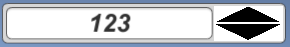
\includegraphics[width=0.6\linewidth]{rc/ui_spinner_layout}
\end{center}

Le widget doit être fonctionnel, mais vous pouvez bien sûr changer/adapter selon vos souhaits le coté esthétique du widget.
De nouveau, vérifiez que le widget contenant la valeur numérique ne soit pas modifiable directement par l'utilisateur.


\ifversionenseignant
\begin{solution}
Ce \texttt{widget} sera composé de deux parties principales : un \texttt{Input Field} et un groupe de deux \texttt{Buttons}, disposés de manière à  laisser seul l'\texttt{Input Field} être redimensionné en fonction des dimensions du parent.	

\subsection{Création du widget}
\begin{itemize}
	\item Dans le \texttt{Canvas} principal, créer un \texttt{Panel} nommé \textit{SpinnerPanel}.
	\item Insérer dans \textit{SpinnerPanel} les enfants suivants :
	\begin{itemize}
		\item \texttt{Input Field (Legacy)}
		\item un \texttt{GameObject} de type \texttt{Empty} nommé \textit{EmptyButtonParent} et dans ce dernier :
		\begin{itemize}
			\item deux \texttt{Buttons (Legacy)} nommés respectivement \textit{ButtonUp} et \textit{ButtonDown}
		\end{itemize}	
	\end{itemize}	
	
	\item Ajouter à \textit{SpinnerPanel} un composant \texttt{Horizontal Layout Group} avec les propriétés:
	\begin{itemize}
		\item \texttt{Padding > Spacing} : $5$
		\item \texttt{Child Alignment} : \textit{Upper Left}
		\item \texttt{Control Child Size} : cocher \textit{Width} et \textit{Height}
		\item \texttt{Child Force Expand} : cocher \textit{Height}
	\end{itemize}	

	\item Dans \texttt{Input Field (Legacy)} :
	\begin{itemize}
		\item \texttt{Composant Input Field}
		\begin{itemize}
			\item propriété \texttt{Interactable} : désactiver pour empêcher l'utilisateur d'écrire dans ce champ
			\item \texttt{Transition > Disabled Color} : cette couleur est gris par défaut, passer cette couleur en blanc et alpha = 255 pour suivre l'illustration du sujet
			\item \texttt{Input Field > Text} : $0$
		\end{itemize}
		\item modifier les enfants
		\begin{itemize}						
			\item \texttt{PlaceHolder > Text > Text} : effacer \textit{"Enter text..."}
			\item \texttt{Text (Legacy) > Character > Font Size} : $30$
			\item \texttt{Text (Legacy) > Paragraph > Alignment} : \textit{Center} et \textit{Middle}
		\end{itemize}		

		\item ajouter un composant \texttt{Layout Element} avec les propriétés
		\begin{itemize}			
			\item \texttt{Min Width} : cocher la case, valeur = $100$
			\item \texttt{Preferred Width} : cocher la case, valeur = $100$
			\item \texttt{Flexible Width} : cocher la case, valeur = $1$
		\end{itemize}	
	\end{itemize}		
	
	 \item Dans \texttt{EmptyButtonParent}, 	ajouter les composants
		\begin{itemize}				
			\item	\texttt{Vertical Layout Group}
			\begin{itemize}
				\item \texttt{Spacing} : $3$
				\item \texttt{Child Alignment} : \textit{Upper Left}
				\item \texttt{Control Child Size} : cocher \textit{Width} et \textit{Height}
				
				\item \texttt{Child Force Expand} : cocher \textit{Height}
			\end{itemize}			
			\item \texttt{Layout Element} (\textbf{ne pas cocher} \texttt{Flexible Width} pour laisser au composant \texttt{Input field (Legacy)} remplir tout l'espace restant)
			\begin{itemize}
				\item \texttt{Min Width} : cocher la case, valeur = $100$
				\item \texttt{Preferred Width} : cocher la case, valeur = $100$
				\item \texttt{Layout Priority} : $1$
			\end{itemize}		
		\end{itemize}				
	
	\item Dans \textit{ButtonUp}
		\begin{itemize}
			\item Ajouter le composant  \texttt{Layout Element} (\textbf{ne pas cocher} \texttt{Flexible Width})
			\begin{itemize}
				\item \texttt{Min Width} : cocher la case, valeur = $100$
				\item \texttt{Preferred Width} : cocher la case, valeur = $100$
				\item \texttt{Layout Priority} : $1$
			\end{itemize}	
			\item Pour associer une image de flèche
			\begin{itemize}
				\item récupérer une image de type PNG et dans l'onglet \texttt{Project}, clic droit et \texttt{Import New Asset...} puis sélectionner le fichier ;
				\item dans \texttt{Project}, sélectionner l'image importée et modifier la propriété \texttt{Texture Type} : \textit{Sprite (2D and UI)} et \texttt{Sprite Mode} : \textit{Single};				
				\item valider le message de création de l'\texttt{Asset} avec le bouton \texttt{Apply} dans l'\texttt{Inspector}.
				\item \textbf{ATTENTION} : les images récupérées doivent suivre un certain format ou bien le message d'erreur apparaît : "\textit{Only textures with width/height multiple of 4 can be compressed to DXT5|BC3 format}".
			\end{itemize}	
			\item dans le composant \texttt{Image}, modifier la propriété
			\begin{itemize}
				\item \texttt{Source Image} en sélectionnant le petit rond à droite du champ et en filtrant la liste avec le nom du fichier
				\item si l'image est mal proportionnée par rapport au \texttt{Button}, on peut modifier la propriété\texttt{ Scale} de son composant \texttt{Rect Transform}
				\item dans l'enfant de type \texttt{Text}, modifier la propriété \texttt{Text > Text} : effacer le texte par défaut "\textit{Button}"
			\end{itemize}
		\end{itemize}	
	\item Dans \textit{ButtonDown} : répéter les opérations entreprises pour \textit{ButtonUp} en choisissant une autre image.
\end{itemize}

\subsection{Script associé à SpinnerPanel}
\begin{boxcode}
\begin{csharpsansbord}
using System;
using System.Collections;
using System.Collections.Generic;
using UnityEngine;
using UnityEngine.UI;
using UnityEngine.EventSystems;

public class SpinnerPannelScript : MonoBehaviour
/*, IPointerDownHandler, IPointerUpHandler, IDragHandler*/
{
	private Button m_ButtonUp, m_ButtonDown;
	private InputField m_InputField;
	
	// Increment laisse au choix de l'utilisateur
	public int m_IncrementStep = 1; 
	
	// Start is called before the first frame update
	void Start()
	{
		m_InputField = gameObject.GetComponentInChildren<InputField>();
		if (m_InputField != null) {
			Debug.Log("Input Field found: " + m_InputField + "name: " +
			m_InputField.name);
		}
		
		Button[] buttons = gameObject.GetComponentsInChildren<Button>();
		if (buttons != null) {
			if (buttons[0].name.Equals("ButtonUp") &&
			buttons[1].name.Equals("ButtonDown")) {
				m_ButtonUp = buttons[0]; 
				m_ButtonDown = buttons[1];
			}
			else if (buttons[1].name.Equals("ButtonUp") &&
			buttons[0].name.Equals("ButtonDown")) {
				m_ButtonUp = buttons[1];
				m_ButtonDown = buttons[0];
			}
			else {
				Debug.Log("Buttons Up and Down not found!");
			}
		}
		else {
			Debug.Log("Buttons not found!");
		}
		
		if (m_ButtonUp != null && m_ButtonDown != null) {
			m_ButtonUp.onClick.AddListener(delegate {
				IncrementField(true);
			});
			m_ButtonDown.onClick.AddListener(delegate {
				IncrementField(false);
			});
		}
	}
\end{csharpsansbord}
\end{boxcode}		

\begin{boxcode}
\begin{csharpsansbord}
	
    // Update is called once per frame
	void Update() { }

	private void IncrementField(bool increment) {
		string m_Text = m_InputField.text;
		try {
			int value = Int32.Parse(m_Text);
			Debug.Log("value = " + value);
			if (increment) {
				value += m_IncrementStep;
			}
			else {
				value -= m_IncrementStep;
			}
			Debug.Log("new value = " + value);
			m_InputField.text = value.ToString();
		}
		catch (FormatException e) {
			Debug.Log(e.Message);
		}
	}
}
\end{csharpsansbord}
\end{boxcode}	
\end{solution}	
\fi 

\section{Aspects avancés sur le système d'événement souris}

%Le système événementiel est en cours de modification, mais 
Nous présentons ici une mécanique pour interagir avec des événements particuliers. Pour cela, consultez le lien suivant qui donne les événements supportés \url{https://docs.unity3d.com/Packages/com.unity.ugui@1.0/manual/SupportedEvents.html}. Nous vous proposons un petit exercice sous forme de tutoriel:
\begin{itemize}
	\item dans un nouveau projet ou une nouvelle \texttt{Scene}\footnote{Dans ce dernier cas, ajouter dans chaque scène un bouton pour permuter entre les scènes.}, ajoutez un \texttt{Panel} occupant l'entièreté du \texttt{Canvas};
	\item modifiez la couleur du \texttt{Panel} pour qu'il soit entièrement transparent;
	\item créez un nouveau script;
	\item au début de ce script, ajoutez la ligne
\begin{lstlisting}
using UnityEngine.EventSystems;	
\end{lstlisting}	
	\item faire hériter le script avec les événements voulus (cf.~lien plus haut). Dans notre exemple, nous allons nous concentrer sur les cliques souris et donc nous prendrons l'interface: \texttt{IPointerClickHandler};
	\item surchargez les fonctions associées aux interfaces. Ici: 
\begin{lstlisting}
public void OnPointerClick(PointerEventData data) { }
\end{lstlisting}		
\end{itemize}


\ifversionenseignant
\begin{solution}
\subsection{Création d'une scène supplémentaire}
	
Pour ajouter une \texttt{Scene} à la \textit{SampleScene} actuelle :
\begin{itemize}
	\item Menu \texttt{File > New Scene > Basic (Built-in)} et cocher \texttt{Load additively} pour que la seconde \texttt{Scene} apparaisse dans la \texttt{Hierarchy}.
	\item Dans la \texttt{Hierarchy}, le nom de la nouvelle \texttt{Scene} est \textit{Untitled}. Cliquer sur le symbole "\textit{3 points verticaux}" à droite de ce nom pour sauvegarder cette \texttt{Scene}, par exemple sous le nom \textit{MouseScene}.
	\item[$\rightarrow$] Les fichiers \textit{MouseScene.unity} et \textit{MouseScene.unity.meta} sont créés.
	\item Dans le \texttt{Project}, double-cliquer sur \texttt{MouseScene} pour la sélectionner et ajouter un \texttt{UI > EventSystem}. \textbf{Attention}, si cette sélection n'est pas faite au préalable, ajouter un \texttt{EventSystem} n'a pas d'effet : on est renvoyé sur le premier ajouté par défaut dans la \texttt{Scene} initiale.
	\item Si une seule des \texttt{Scenes} apparaît dans la \texttt{Hierarchy}, déplacer l'autre depuis le \texttt{Project} vers la \texttt{Hierarchy} pour la faire apparaître.
\end{itemize}	
		
\textbf{Important}: Dans le menu \texttt{File > Build Profiles}, vérifier dans \texttt{Platforms > Scene List} que toutes les scènes sont bien cochées. Éventuellement, cliquer sur \texttt{Add Open Scenes} pour afficher les \texttt{Scenes} dans la listes "\textit{Scenes In Build}".\\

Remarque : les deux \texttt{Cameras} ont la même valeur de propriété \texttt{Camera > Depth = $-1$}. Dans le mode \texttt{Game}, c'est la \texttt{Camera} la plus récente (celle de \textit{MouseScene}) qui est affichée par défaut. Pour revenir à la vue sur \textit{SampleScene}, il faut augmenter la valeur de ce champ pour \textit{Main Camera}.

Important: En complément de la remarque précédente, on peut spécifier la \texttt{Scene} active en cliquant sur le nom d'une \texttt{Scene}, puis \texttt{bouton droit > Set Active Scene}.

\subsubsection{Peuplement de la nouvelle Scene}
\begin{itemize}	
	\item  Ajouter un bouton dans le \texttt{Canvas} de \textit{SampleScene} : \texttt{UI > Legacy > Button (Legacy)}
	\begin{itemize}
		\item nommer ce bouton \textit{ButtonSwitchToMouseScene}
		\item modifier son enfant \texttt{Text (Legacy)}
		\begin{itemize}
			\item Composant \texttt{Text}
			\begin{itemize}
				\item propriété \texttt{Text} = \textit{Set MouseScene}
				\item  propriété \texttt{Character > Font Size} = $32$
			\end{itemize}	
			\item Composant \texttt{Rect Transform}
			\begin{itemize}
				\item \texttt{ancre} \textit{bottom left}
				\item \texttt{Pos X = 50 ; Pos Y = 35 ; Pos Z = 0}
				\item 	\texttt{Width = 280 ; Height = 45}
				\item[$\Rightarrow$] au besoin, changer ces valeurs pour ne pas empiéter sur les autres enfants du \texttt{Panel}.
			\end{itemize}	
		\end{itemize}
	\end{itemize}

	\item Créer un nouveau \texttt{Canvas} dans \textit{MouseScene}. \textbf{Attention}~: si on duplique le \texttt{Canvas} de \texttt{SampleScene} pour le déplacer dans \texttt{MouseScene}, un message d'erreur peut s'afficher, comme quoi la \texttt{Main~Camera} de \texttt{SampleScene} est également référencée dans \texttt{MouseScene} $\Rightarrow$ à éviter.
	
	\item Dans \textit{MouseScene}:
	\begin{itemize}
		\item Supprimer si on le souhaite \textit{ComplexSliderJoli} ou \textit{SpinnerPanel}, ou bien les déplacer, pour modifier l'allure du \texttt{Canvas}.
	
		\item Renommer le \texttt{Button} dupliqué en  \textit{ButtonSwitchToSampleScene}.
	
		\item Soit dans \textit{SpinnerPanel}, soit dans un nouveau \texttt{Panel}, modifier
	\begin{itemize}
		\item 	Composant \texttt{Image}: modifier la propriété \texttt{Color} pour mettre la valeur du canal alpha à 0 : le \texttt{Panel} devient complètement transparent.
	\end{itemize}	
	\item \texttt{Button} \textit{ButtonSwitchToSampleScene}
	\begin{itemize}
		\item Enfant \texttt{Text > Text} : propriété \texttt{Text} = \textit{Set SampleScene}
	\end{itemize}
\end{itemize}	
\end{itemize}

\subsubsection{Script de permutation de Scenes}

Associer le script suivant aux \texttt{Buttons}  \textit{ButtonSwitchToMouseScene} et \textit{ButtonSwitchToSampleScene}.


\begin{boxcode}
\begin{csharpsansbord}
using UnityEngine;
using UnityEngine.UI;
using UnityEngine.EventSystems;
using UnityEngine.SceneManagement;

// Charge une des scenes du projet.
// Ce script est associe a tous les boutons (un par scene)
// permettant de selectionner une autre scene

// ATTENTION : un GameObject "EventSystem" doit etre place dans CHAQUE scene
// pour que les iteractions soient prises en compte.

// Source : https://www.youtube.com/watch?v=PpIkrff7bKU
public class SelectSceneScript : MonoBehaviour
{
	private Button m_Button;
	
	// Start is called before the first frame update
	void Start()
	{
		m_Button = gameObject.GetComponent<Button>();
		if (m_Button == null) {
			Debug.Log("m_Button = null");
		}
		else {
			Debug.Log("m_Button " + m_Button.name + " found.");
		}
		m_Button.onClick.AddListener(delegate {
			SetOtherScene();
		});
	}
	
	// Update is called once per frame
	void Update() {	}
	
	private void SetOtherScene() {
		Debug.Log("Enter SetOtherScene");
		if (m_Button.name.ToString().Equals("ButtonSwitchToMouseScene")) {
			SceneManager.LoadScene(SceneManager.GetActiveScene().buildIndex + 1);
			Debug.Log("Selected button : ButtonSwitchToMouseScene");
		}
		else if (m_Button.name.ToString().Equals("ButtonSwitchToSampleScene")) {
			SceneManager.LoadScene(SceneManager.GetActiveScene().buildIndex - 1);
			Debug.Log("Selected button : ButtonSwitchToSmapleScene");
		}
		else {
			Debug.Log("Error SetOtherScene");
		}
	}
}

\end{csharpsansbord}
\end{boxcode}		

\textcolor{red}{\textbf{ATTENTION} : parfois, le contenu de la seconde \texttt{Scene} dans la \texttt{Hierarchy} semble disparaître, mais tout revient dans l'ordre en mode \texttt{Game}, quand on permute entre les deux \texttt{Scenes} ???. \\
On peut ouvrir chaque \texttt{Scene} indépendamment dans le menu \texttt{File > Open  [Recent] Scene}}.



\subsection{Gestion de la souris}
Associer le script  suivant dans un Panel ou l'un de ses enfants (peu importe la \texttt{Scene}, du moment qu'elle contienne un \texttt{EventSystem}).

\begin{boxcode}
\begin{csharpsansbord}
using UnityEngine;
using UnityEngine.UI;
using UnityEngine.EventSystems;

// Affiche les coordonnees de la souris à chaque clic
public class PanelMouseScript : MonoBehaviour, IPointerClickHandler
{
	public void OnPointerClick(PointerEventData data)
	{
		Debug.Log("OnPointerClick " + data);
	}
}
\end{csharpsansbord}
\end{boxcode}

Le message associé à \texttt{OnPointerClick} apparaît au-dessous de l'onglet \texttt{Console}.
\end{solution}	
\fi 



Normalement, les événements gérés par cette mécanique réagissent par défaut et vous pouvez le vérifier avec des messages de \texttt{Log}. À présent, nous souhaitons réaliser les traitements suivants.
\begin{enumerate}
	\item  Lorsque nous cliquons sur une zone de l'écran, nous voulons créer à la volée un \texttt{widget} de notre choix à l'écran en tant que fils de notre \texttt{Panel} initial (n'oubliez pas qu'un \texttt{widget} UI doit avoir comme parent un \texttt{Canvas}). On suppose que dans le script, on connaît à l'avance le \texttt{widget} qui sera cloné.
	Pour réaliser cela, consultez  la page \url{https://docs.unity3d.com/ScriptReference/Object.Instantiate.html}. \\	
%%	Réalisez un exemple simple. Que remarquez-vous sur le pivot de vos ajouts?
	
	
\ifversionenseignant
\begin{solution}
%	\subsection{Ajout de widget}
Dans l'une des \texttt{Scenes}, par exemple \textit{MouseScene}, insérer dans le \texttt{Canvas > Panel} un \texttt{widget} quelconque, par exemple un \texttt{Button} nommé \textit{ButtonToClone}.	\\

Puis associer le script suivant au \texttt{Canvas > Panel}.

\begin{boxcode}
\begin{csharpsansbord}
using UnityEngine;
using UnityEngine.UI;
using UnityEngine.EventSystems;

// Script associe a un Panel
// Clone un widget choisi par l'utilisateur lors d'un clic de souris.
// Ce widget sera integre comme fils du Panel.
// La position du clone est determinee par la position du curseur de la souris 
public class CloneWidgetScript : MonoBehaviour, IPointerClickHandler
{
	private static string TAG = "CW - ";
	private Camera m_Camera;
	public GameObject m_Widget; // Widget selectionne par l'utilisateur
	
	void Start() {
		// https://docs.unity3d.com/ScriptReference/Camera.html
		// The first enabled Camera component that is tagged "MainCamera"
		//  (Read Only).
		m_Camera = Camera.main;
		if (m_Camera == null) {	Debug.Log(TAG + "Camera not found !");	}
		
		Button[] buttons = gameObject.GetComponentsInChildren<Button>();
		if (buttons != null) {
			int i = 0;
			while (i < buttons.Length &&
			(! buttons[i].name.Equals("ButtonToClone"))) { i++;	}
			
			if (i == buttons.Length) {
				Debug.Log(TAG + "Button to clone not found!");
				m_Widget = null;
			}
			else {
				m_Widget = buttons[i].gameObject;
				Debug.Log(TAG + m_Widget.name + " found!");				
			}
		}
	}
	
	public void OnPointerClick(PointerEventData data)
	{
		Debug.Log(TAG + "OnPointerClick " + data);		
		
		if (m_Widget != null) {
			Vector2 localPoint = new Vector2(data.position.x, data.position.y);
			Debug.Log(TAG + "Local point: " + localPoint);
			
			GameObject obj = Instantiate(m_Widget,
			localPoint,
			Quaternion.identity,
			gameObject.transform);
		}
		else {
			Debug.Log(TAG + "Pas de widget selectionne !");
		}
	}
}

\end{csharpsansbord}
\end{boxcode}

\end{solution}	
\fi 
		
	
	\item Enfin, vous êtes prêt à créer un script \texttt{ResizeWidget} qui consiste à agrandir en largeur/hauteur un \texttt{widget} quelconque en faisant un drag sur ce \texttt{widget}.
	
\ifversionenseignant
\begin{solution}
On associe le script suivant au dernier \texttt{Button} créé dans \textit{MouseScene}: \textit{ButtonToClone} (mais on pourrait utiliser n'importe quel widget).
	
\begin{boxcode}
\begin{csharpsansbord}
using UnityEngine;
using UnityEngine.UI;
using UnityEngine.EventSystems;

// Redimensionne le Widget associe a ce script, selon le "drag" de souris
// Les directions "Droite" et "Bas" permettent de grossir le widget
public class ResizeWidgetScript : MonoBehaviour, IPointerDownHandler,
   IPointerUpHandler, IDragHandler
{
	private Vector2 previousPointerPosition;
	private Vector2 currentPointerPosition;
	private RectTransform rectTransform;
	private static string TAG = "RW - ";
	
	// Use Awake to initialize variables or states before the application starts.	
	private void Awake() { rectTransform = GetComponent<RectTransform>(); }
	
	public void OnPointerDown(PointerEventData data) {
		Debug.Log(TAG + "OnPointerDown " + data);
	}
	
	public void OnPointerUp(PointerEventData eventData) {
		Debug.Log(TAG + "OnPointerUp " + eventData);
	}
	
	public void OnDrag(PointerEventData data) {
		Debug.Log(TAG + "OnDrag " + data);
		rectTransform = GetComponent<RectTransform>();
		
		if (rectTransform == null) {
			Debug.Log(TAG + "RectTransform not found !");
			return;
		}
		
// https://docs.unity3d.com/ScriptReference/RectTransform-sizeDelta.html
		Vector2 sizeDelta = rectTransform.sizeDelta;
		Debug.Log(TAG + "Current Size: " + sizeDelta);
		
// https://docs.unity3d.com/ScriptReference/RectTransformUtility.ScreenPointToLocalPointInRectangle.html
		RectTransformUtility.
		ScreenPointToLocalPointInRectangle(rectTransform,
			data.position,
			data.pressEventCamera,
			out currentPointerPosition);
		Vector2 resizeValue = currentPointerPosition - previousPointerPosition;
		
		Debug.Log(TAG + "Resize: " + resizeValue);
		
		sizeDelta += new Vector2(resizeValue.x, -resizeValue.y);
		
		rectTransform.sizeDelta = sizeDelta;
		Debug.Log(TAG + "New size: " + rectTransform);
		
		previousPointerPosition = currentPointerPosition;
	}
}	
\end{csharpsansbord}
\end{boxcode}

\end{solution}	
\fi 

	
\end{enumerate}
\end{document}
